\documentclass[cn,11pt,english,black,simple,device=ppt]{elegantbook}

\def\mainclass{main}

\title{CMOS 模拟集成电路设计}
% \subtitle{数字设计初步}

\author{Pannenets.F}
% \institute{微电子学院}
\date{\today}
% \version{4}
% \bioinfo{分类}{笔记}

\extrainfo{Je reviendrai et je serai des millions. —— <<Spartacus>>}
\setcounter{tocdepth}{3}

\lstset{
  mathescape = false}
% \logo{logo-blue.png}
% \cover{logo.jpg}

% 微分号
\newcommand{\dd}[1]{\mathrm{d}#1}
\newcommand{\pp}[1]{\partial{}#1}

\newcommand{\homep}[1]{\section*{Problem #1}}

% FT LT ZT
\newcommand{\ft}[1]{\mathscr{F}[#1]}
\newcommand{\fta}{\xrightarrow{\mathscr{F}}}
\newcommand{\lt}[1]{\mathscr{L}[#1]}
\newcommand{\lta}{\xrightarrow{\mathscr{L}}}
\newcommand{\zt}[1]{\mathscr{Z}[#1]}
\newcommand{\zta}{\xrightarrow{\mathscr{Z}}}

% 积分求和号

\newcommand{\dsum}{\displaystyle\sum}
\newcommand{\aint}{\int_{-\infty}^{+\infty}}

% 简易图片插入
\newcommand{\qfig}[3][nolabel]{
  \begin{figure}[!htb]
      \centering
      \includegraphics[width=0.6\textwidth]{#2}
      \caption{#3}
      \label{\chapname :#1}
  \end{figure}
}

% 表格
\renewcommand\arraystretch{1.5}


% 日期


\begin{document}

\maketitle
\frontmatter

\tableofcontents

\mainmatter

\part{课件}

\chapter{MOSFET}

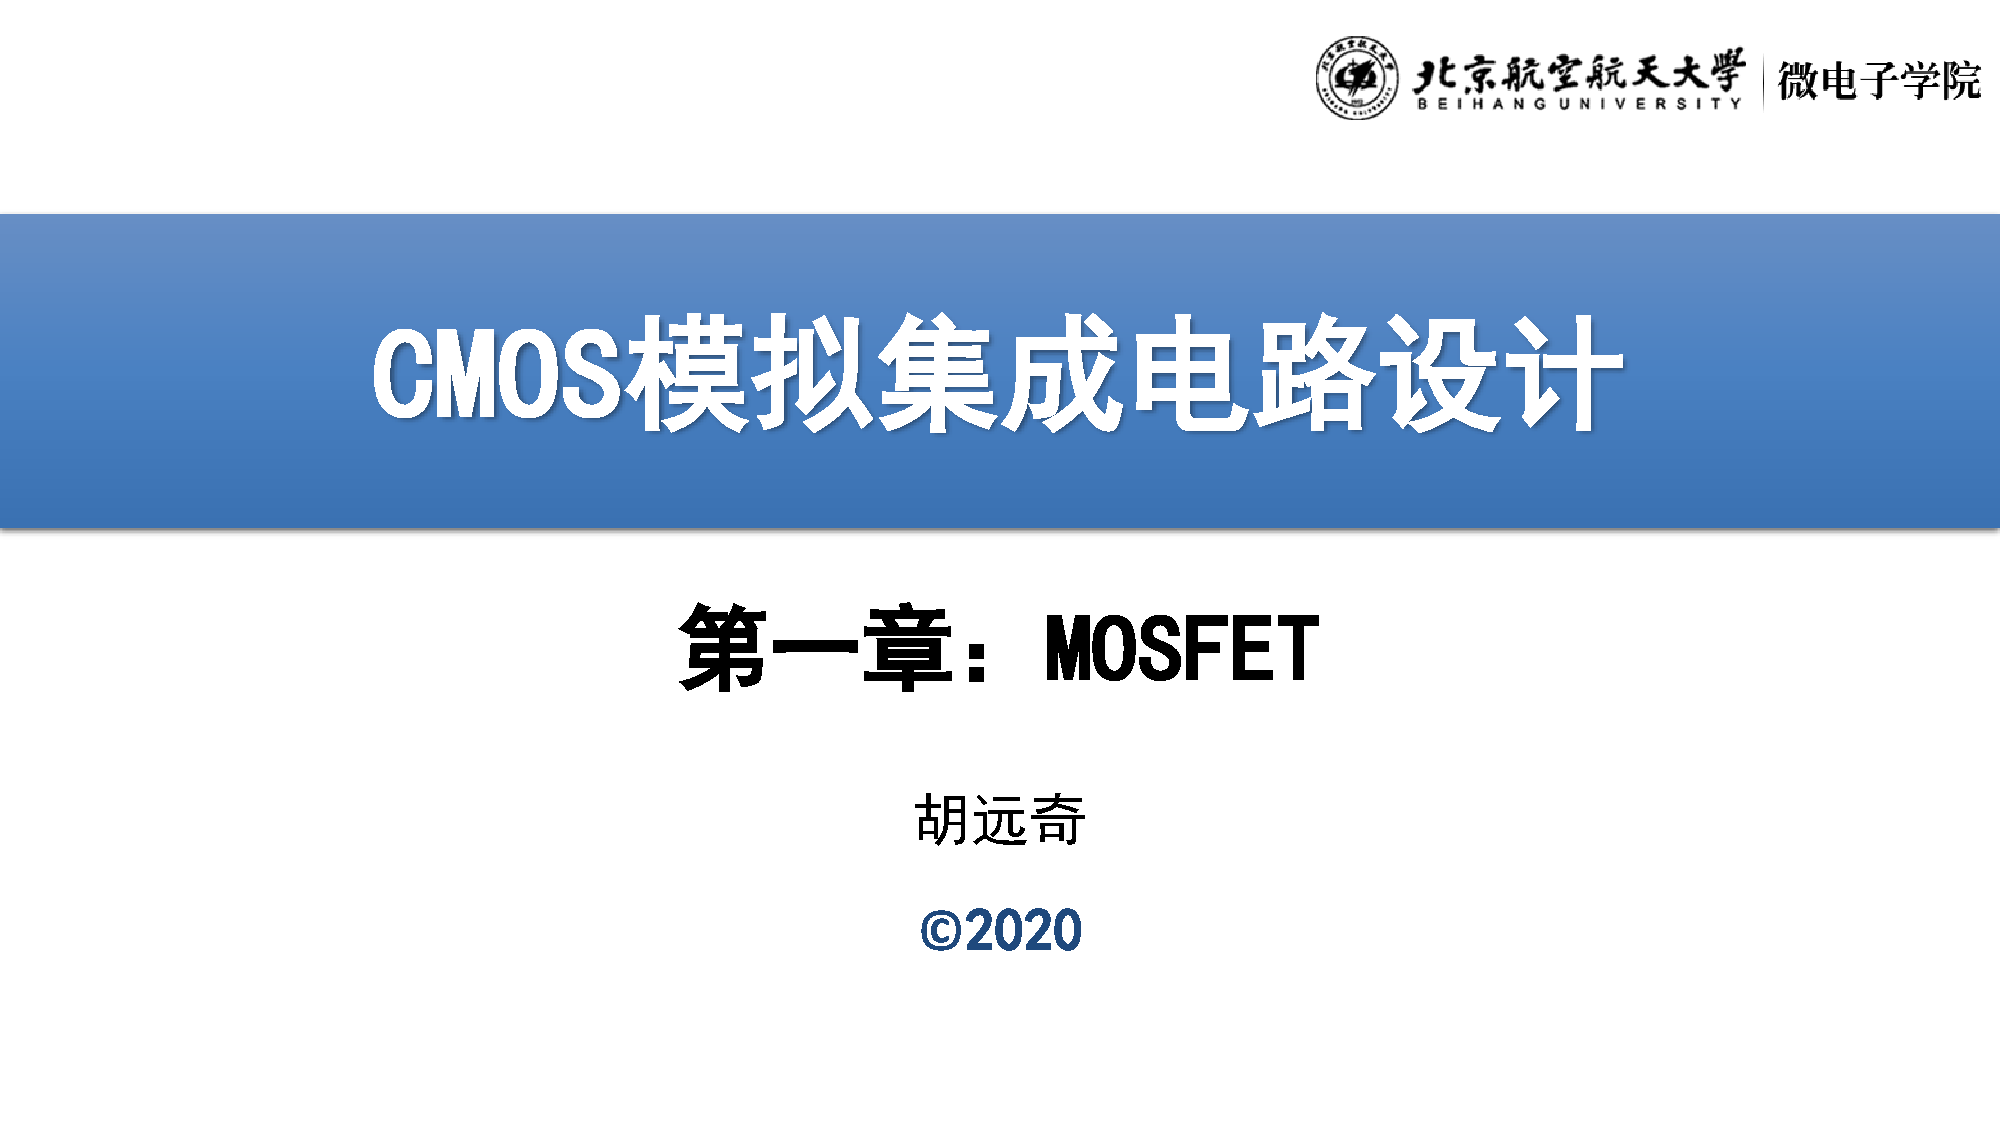
\includepdf[pages=-]{chap/chap01.pdf}

\chapter{模拟电路基本组成}


\includepdf[pages=-]{chap/chap02.pdf}

\chapter{噪声}


\includepdf[pages=-]{chap/chap03.pdf}

\chapter{失配}


\includepdf[pages=-]{chap/chap04.pdf}

\chapter{运放}

\includepdf[pages=-]{chap/chap05.pdf}

\chapter{知识总结1-5}

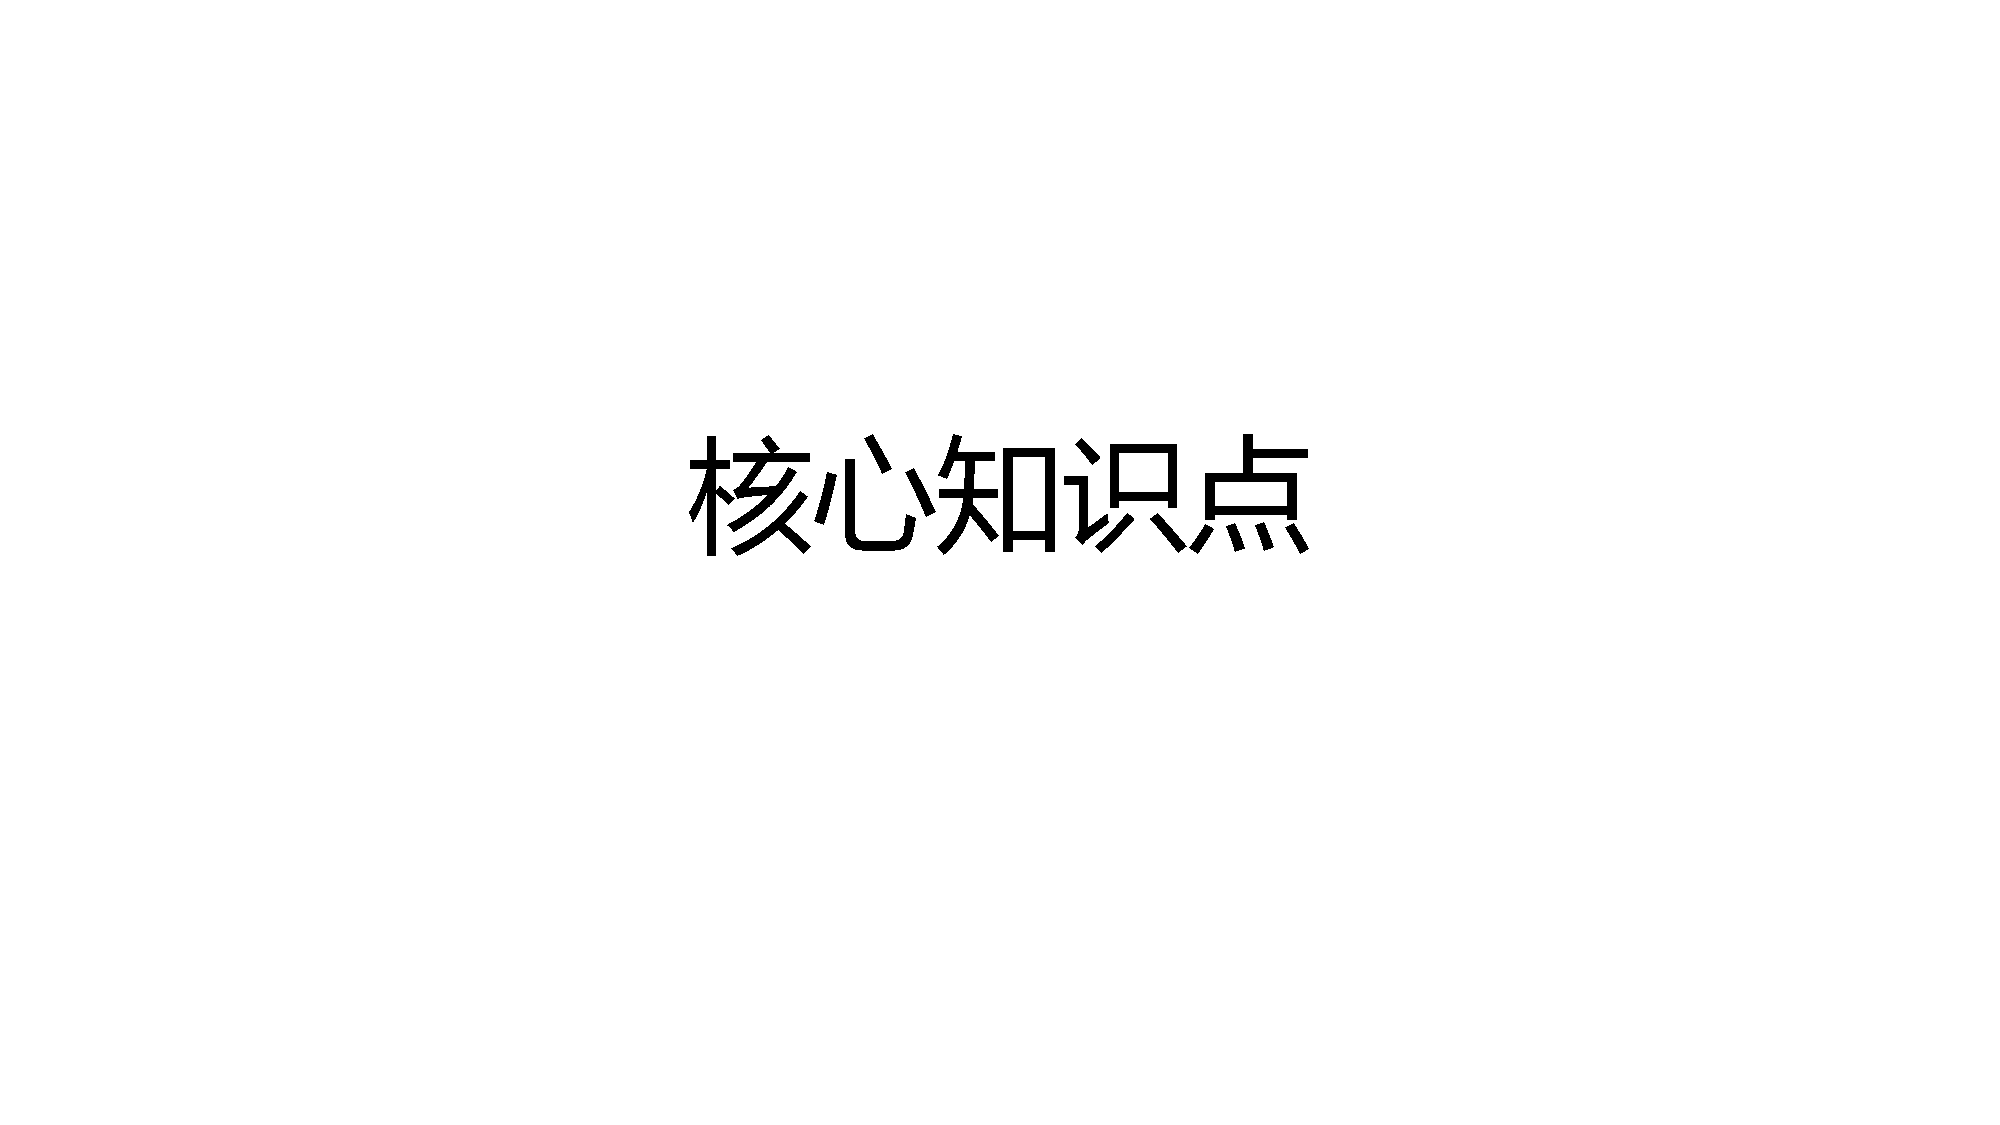
\includepdf[pages=-]{chap/核心知识点1-5.pdf}

\chapter{全差分放大器}


\includepdf[pages=-]{chap/chap07.pdf}

\chapter{轨到轨}


\includepdf[pages=-]{chap/chap08.pdf}

\chapter{Class A-B}

\chapter{全差分放大器}


\includepdf[pages=-]{chap/chap09.pdf}

\chapter{ADC \& DAC} 


\includepdf[pages=-]{chap/chap10.pdf} 

\part{作业反馈}

\chapter{HW01-02}

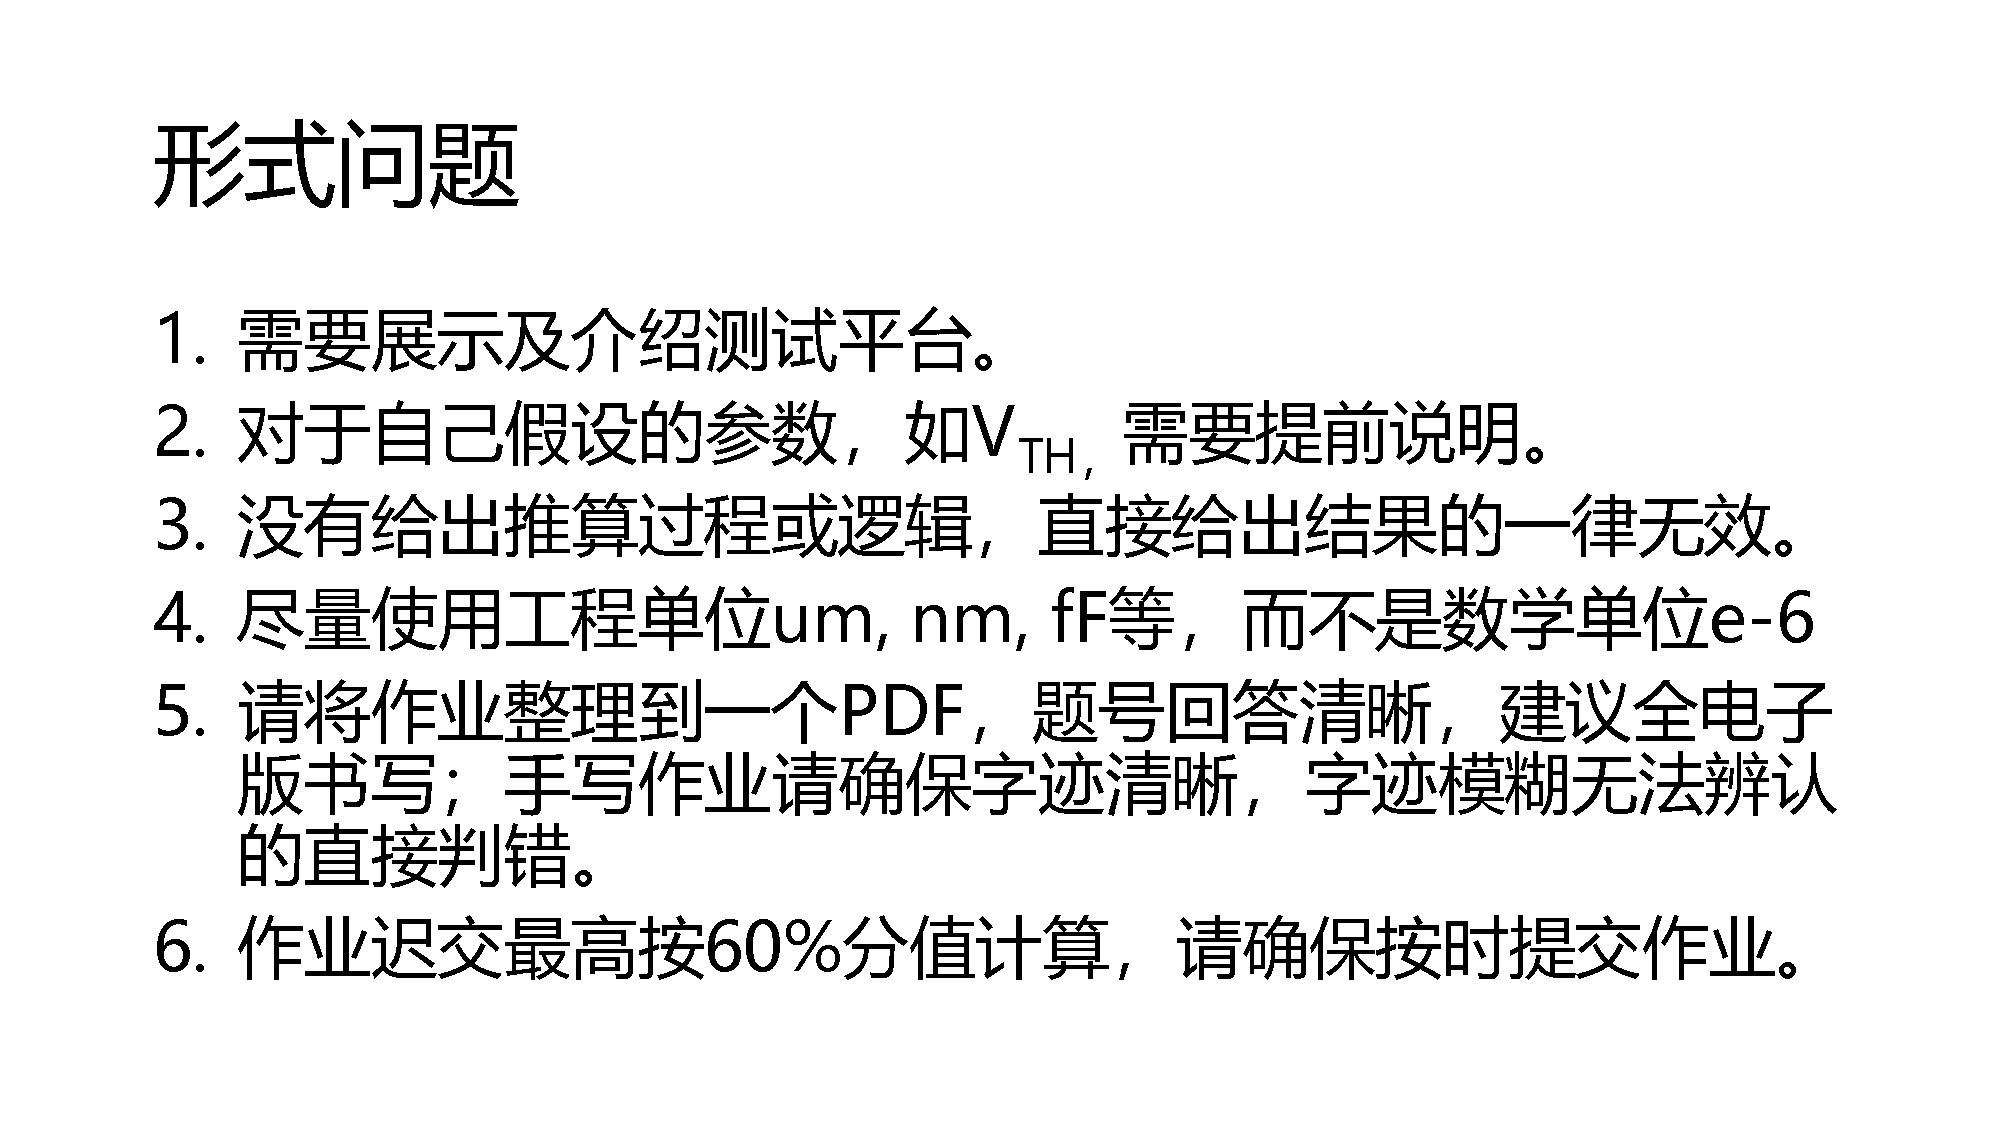
\includepdf[pages=-]{chap/作业反馈1-2.pdf} 

\chapter{HW03}

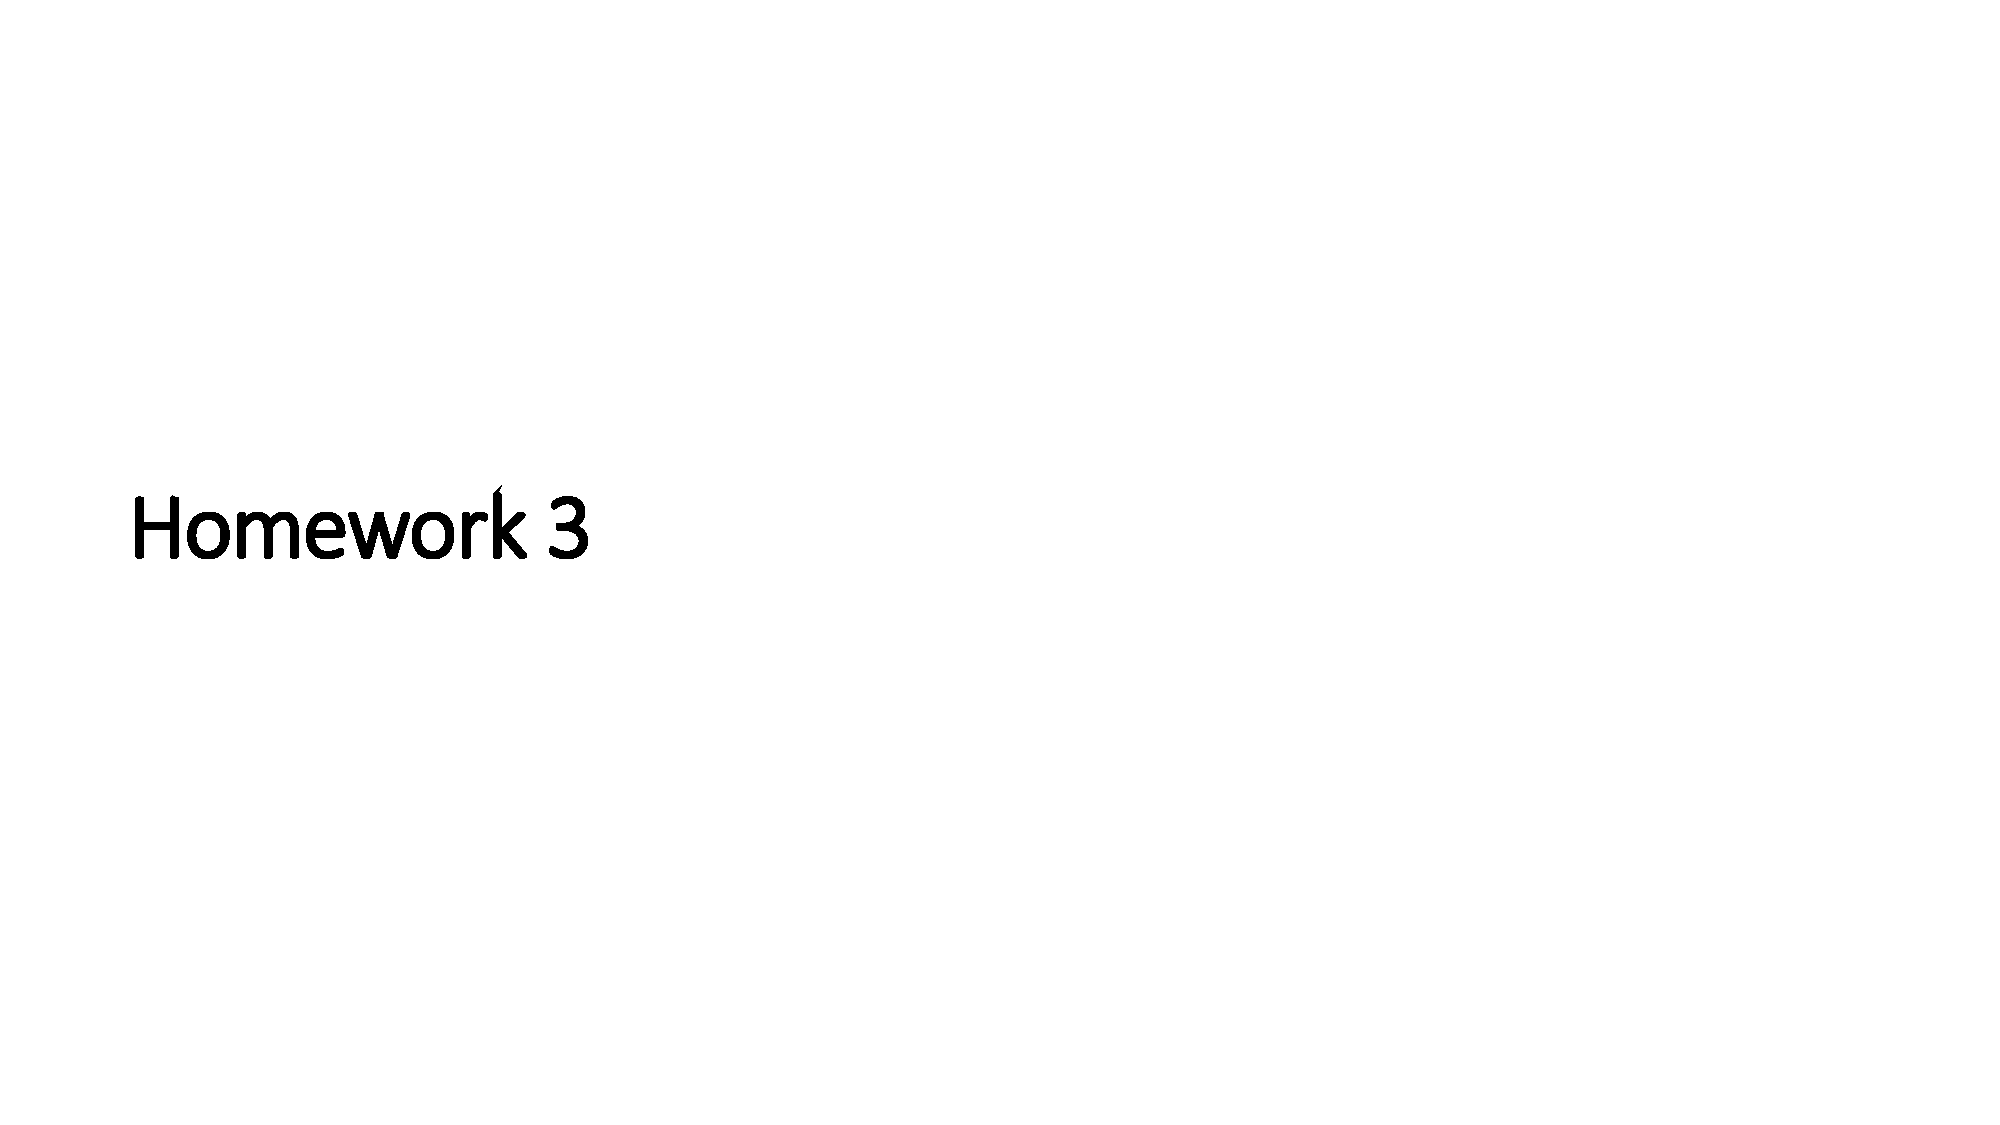
\includepdf[pages=-]{chap/作业反馈3.pdf} 

\chapter{HW04-05}

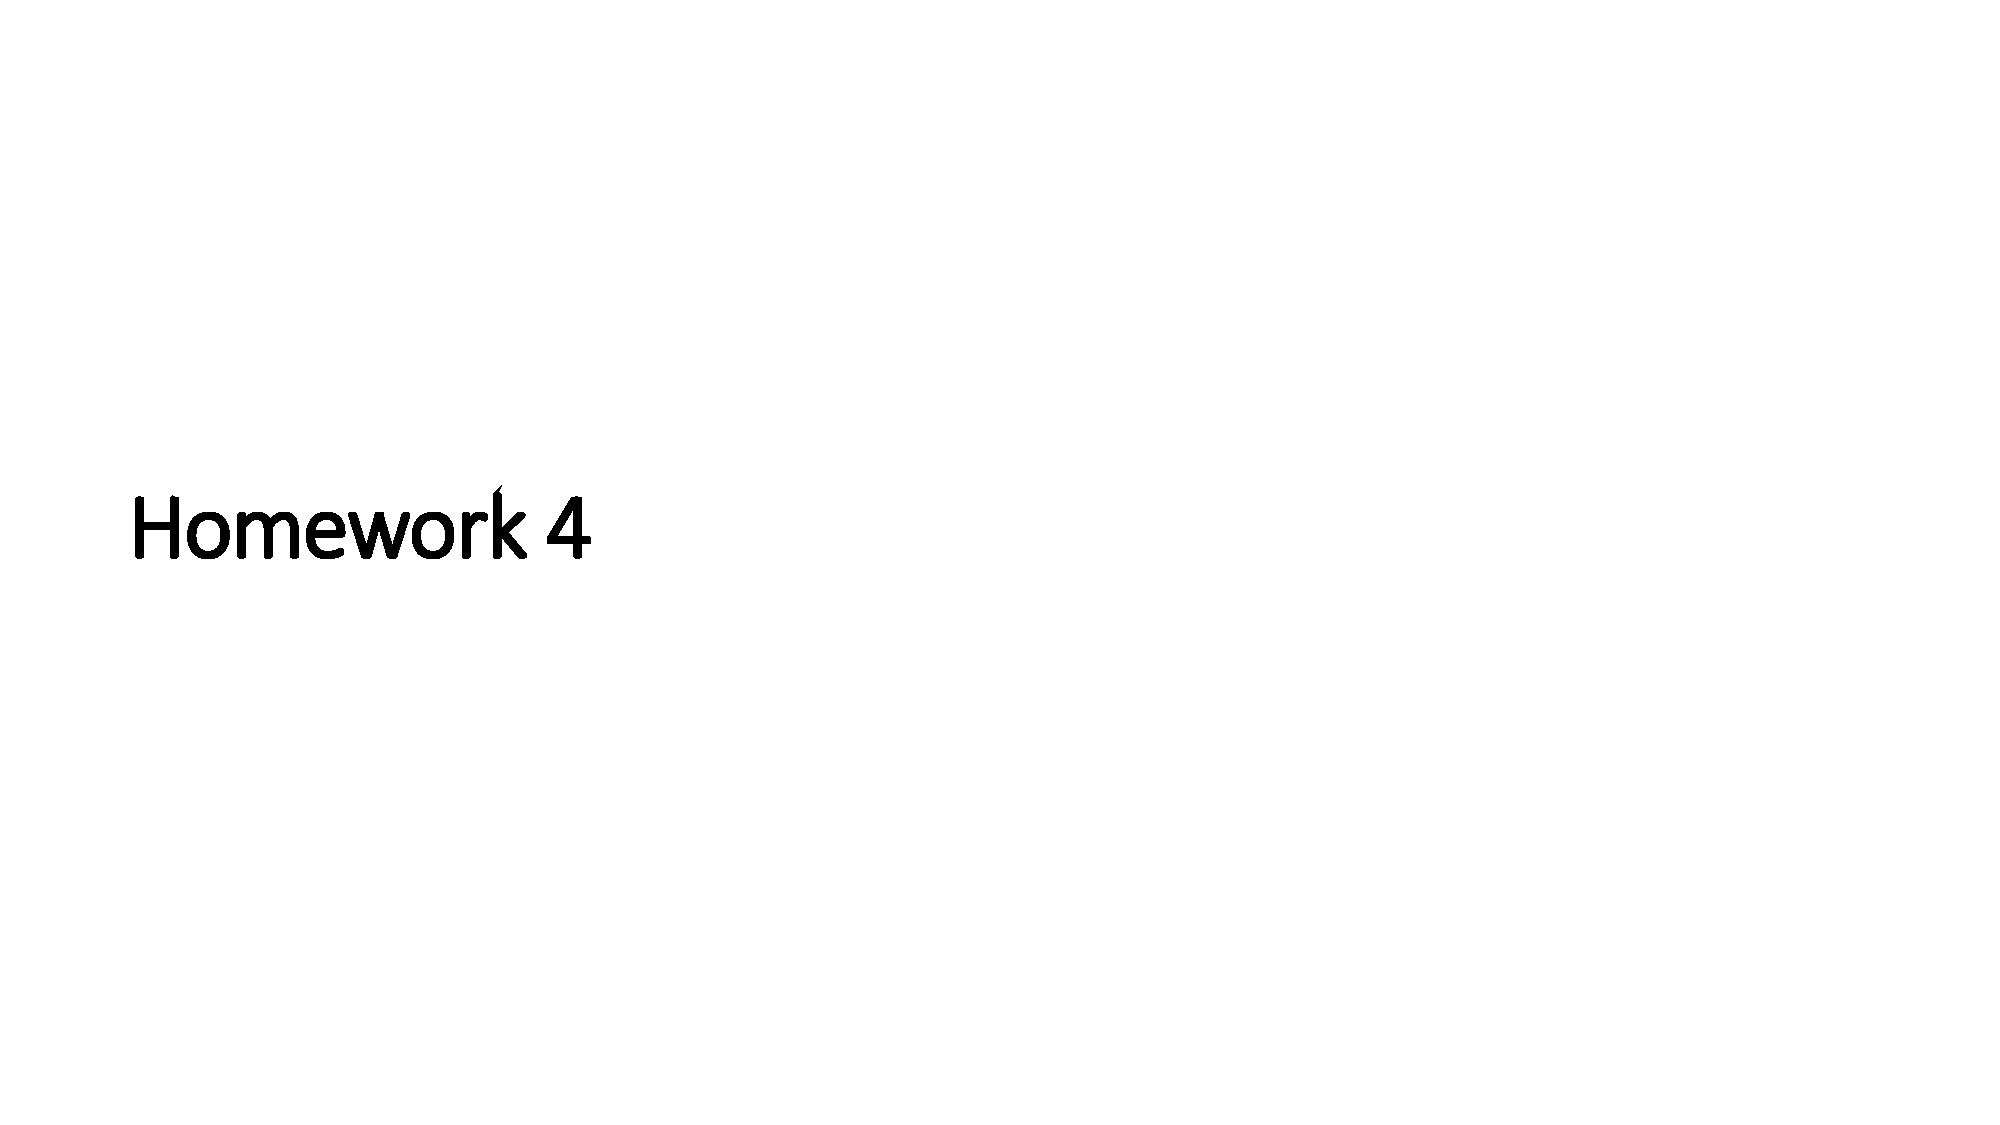
\includepdf[pages=-]{chap/作业反馈4-5.pdf} 

\chapter{HW06}

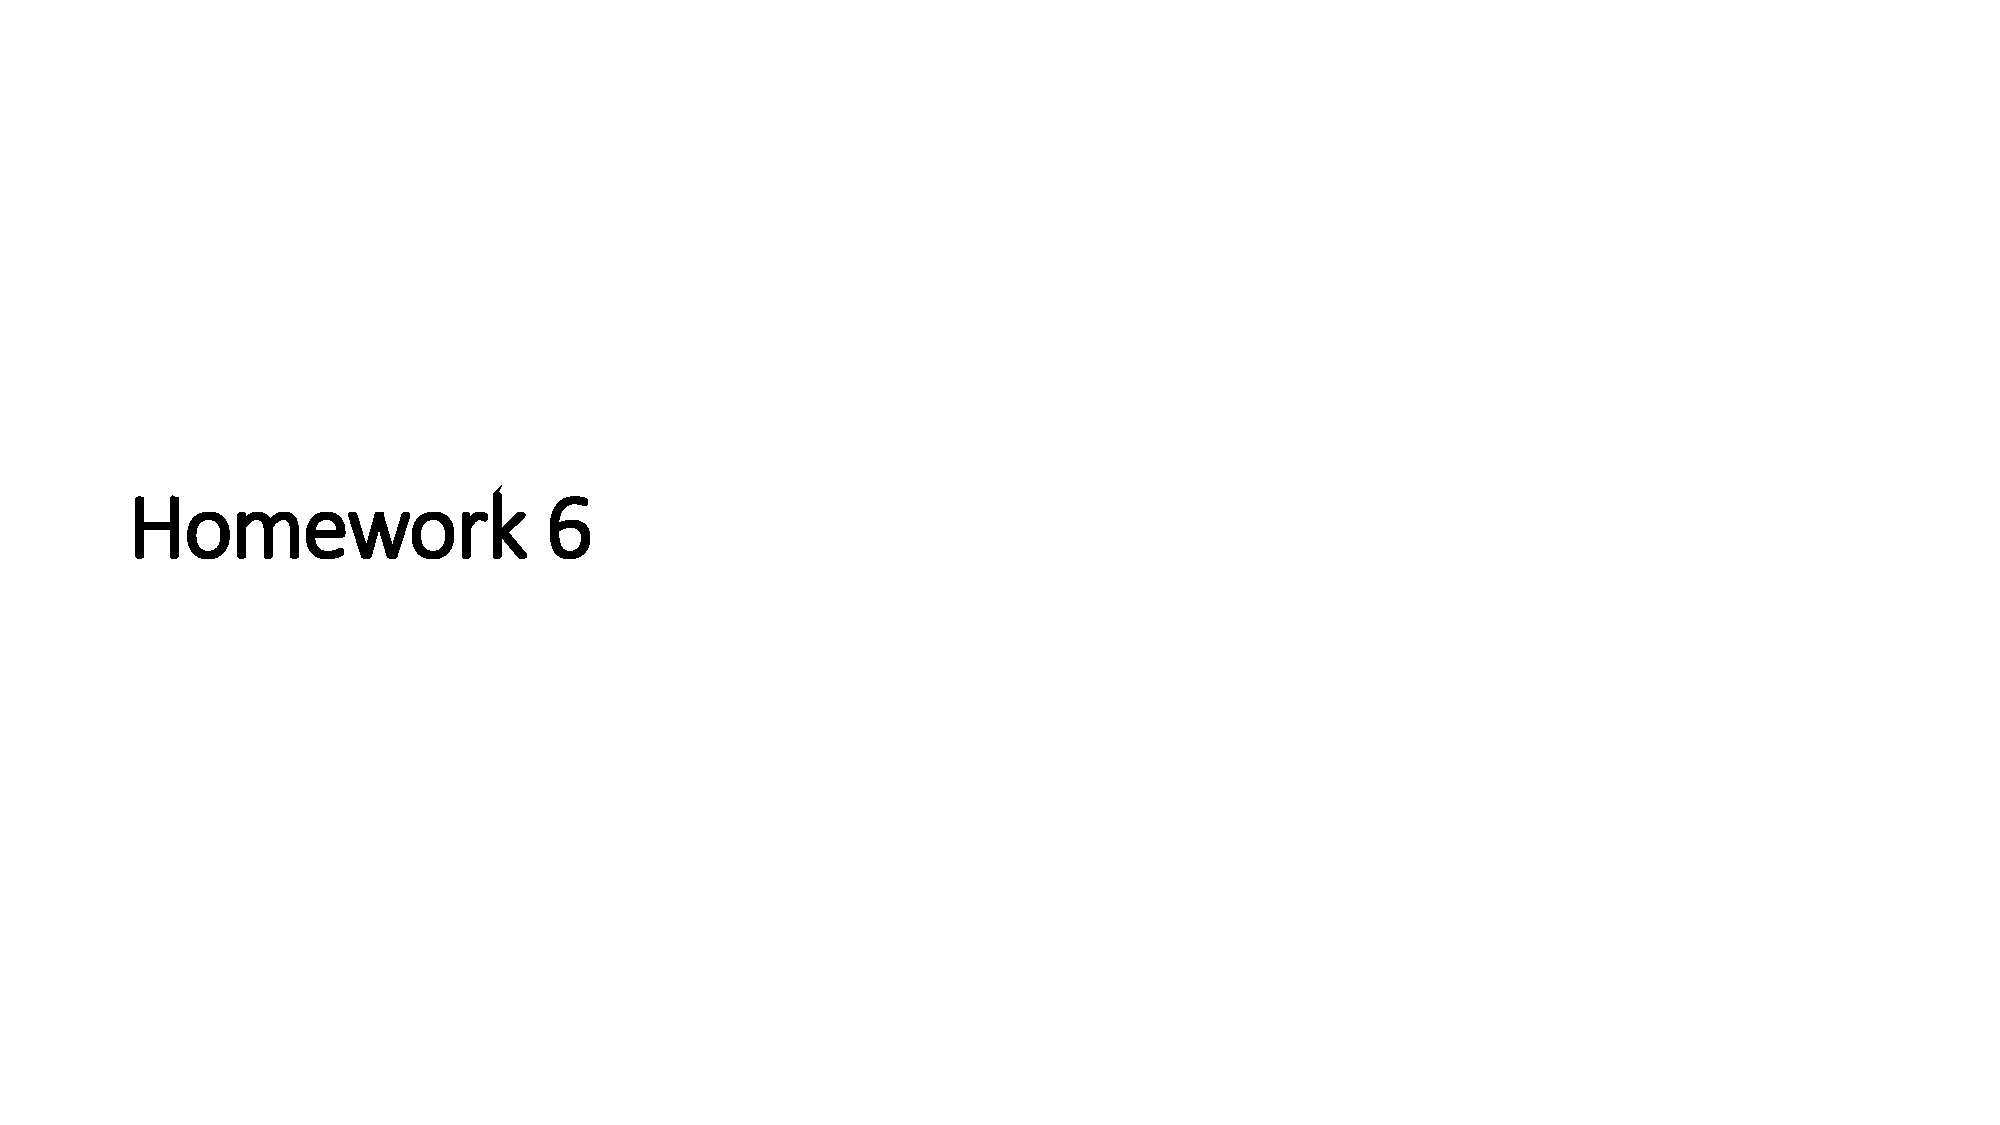
\includepdf[pages=-]{chap/作业反馈6.pdf} 

\chapter{HW07}

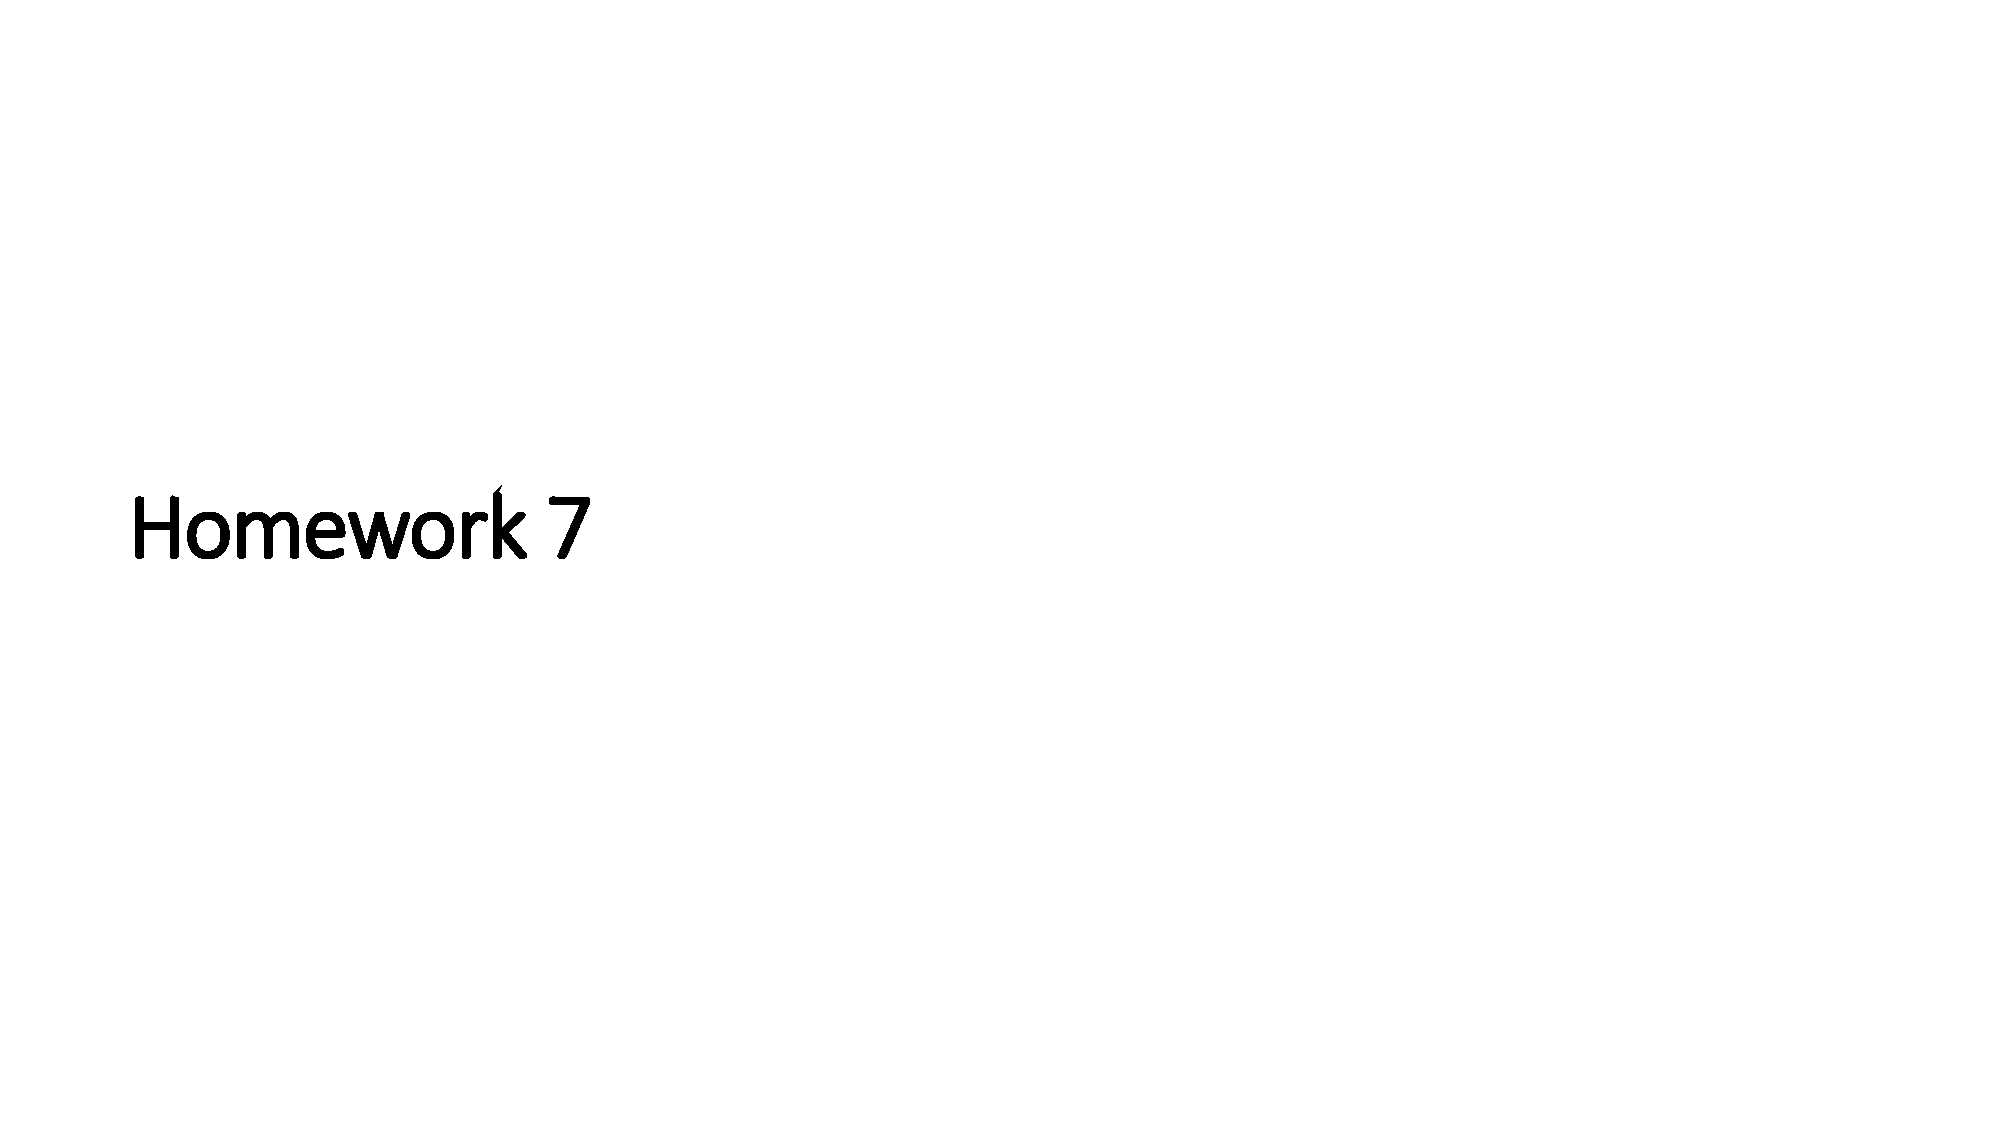
\includepdf[pages=-]{chap/作业反馈7.pdf} 

\chapter{HW08}

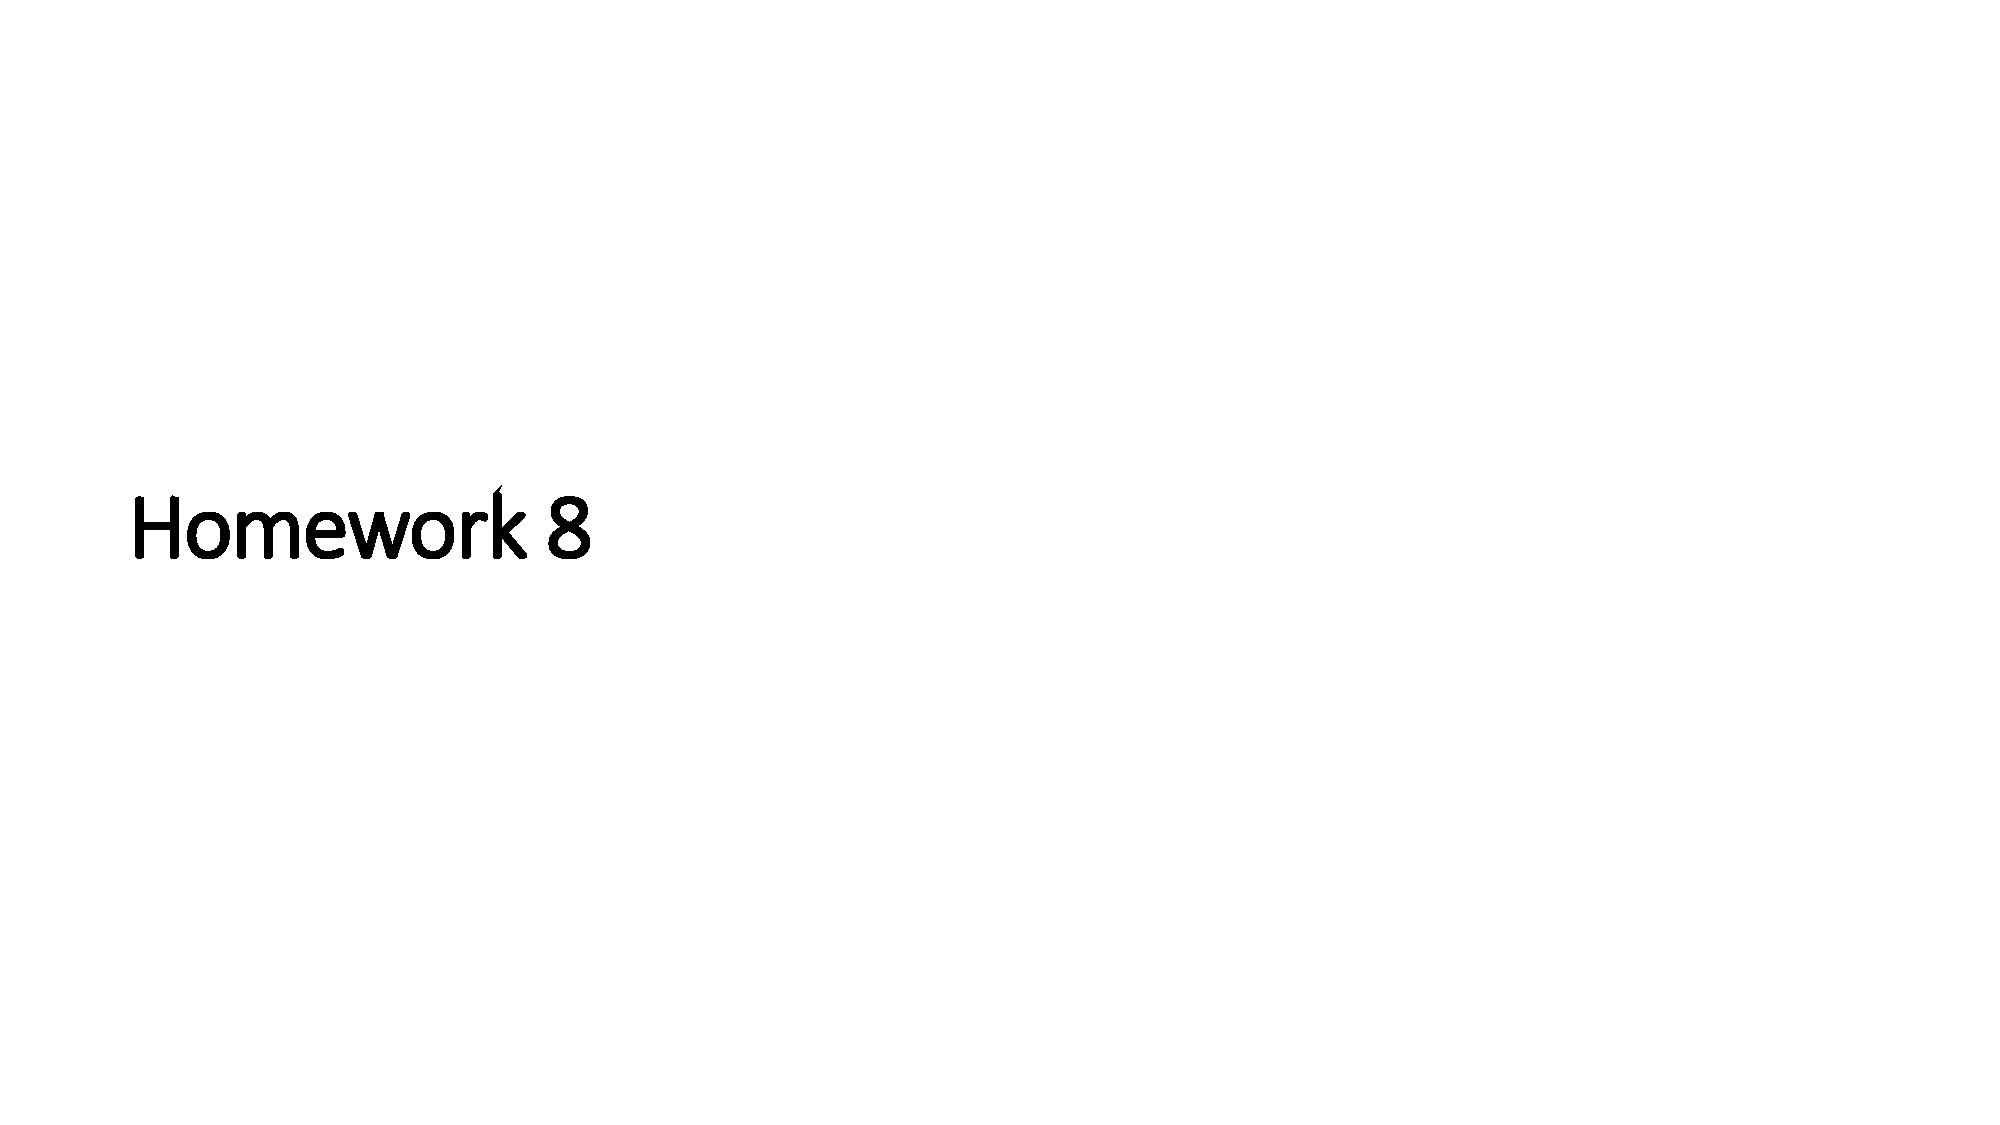
\includepdf[pages=-]{chap/作业反馈8.pdf} 

\part{教程}

\chapter{Aether 入门教程}

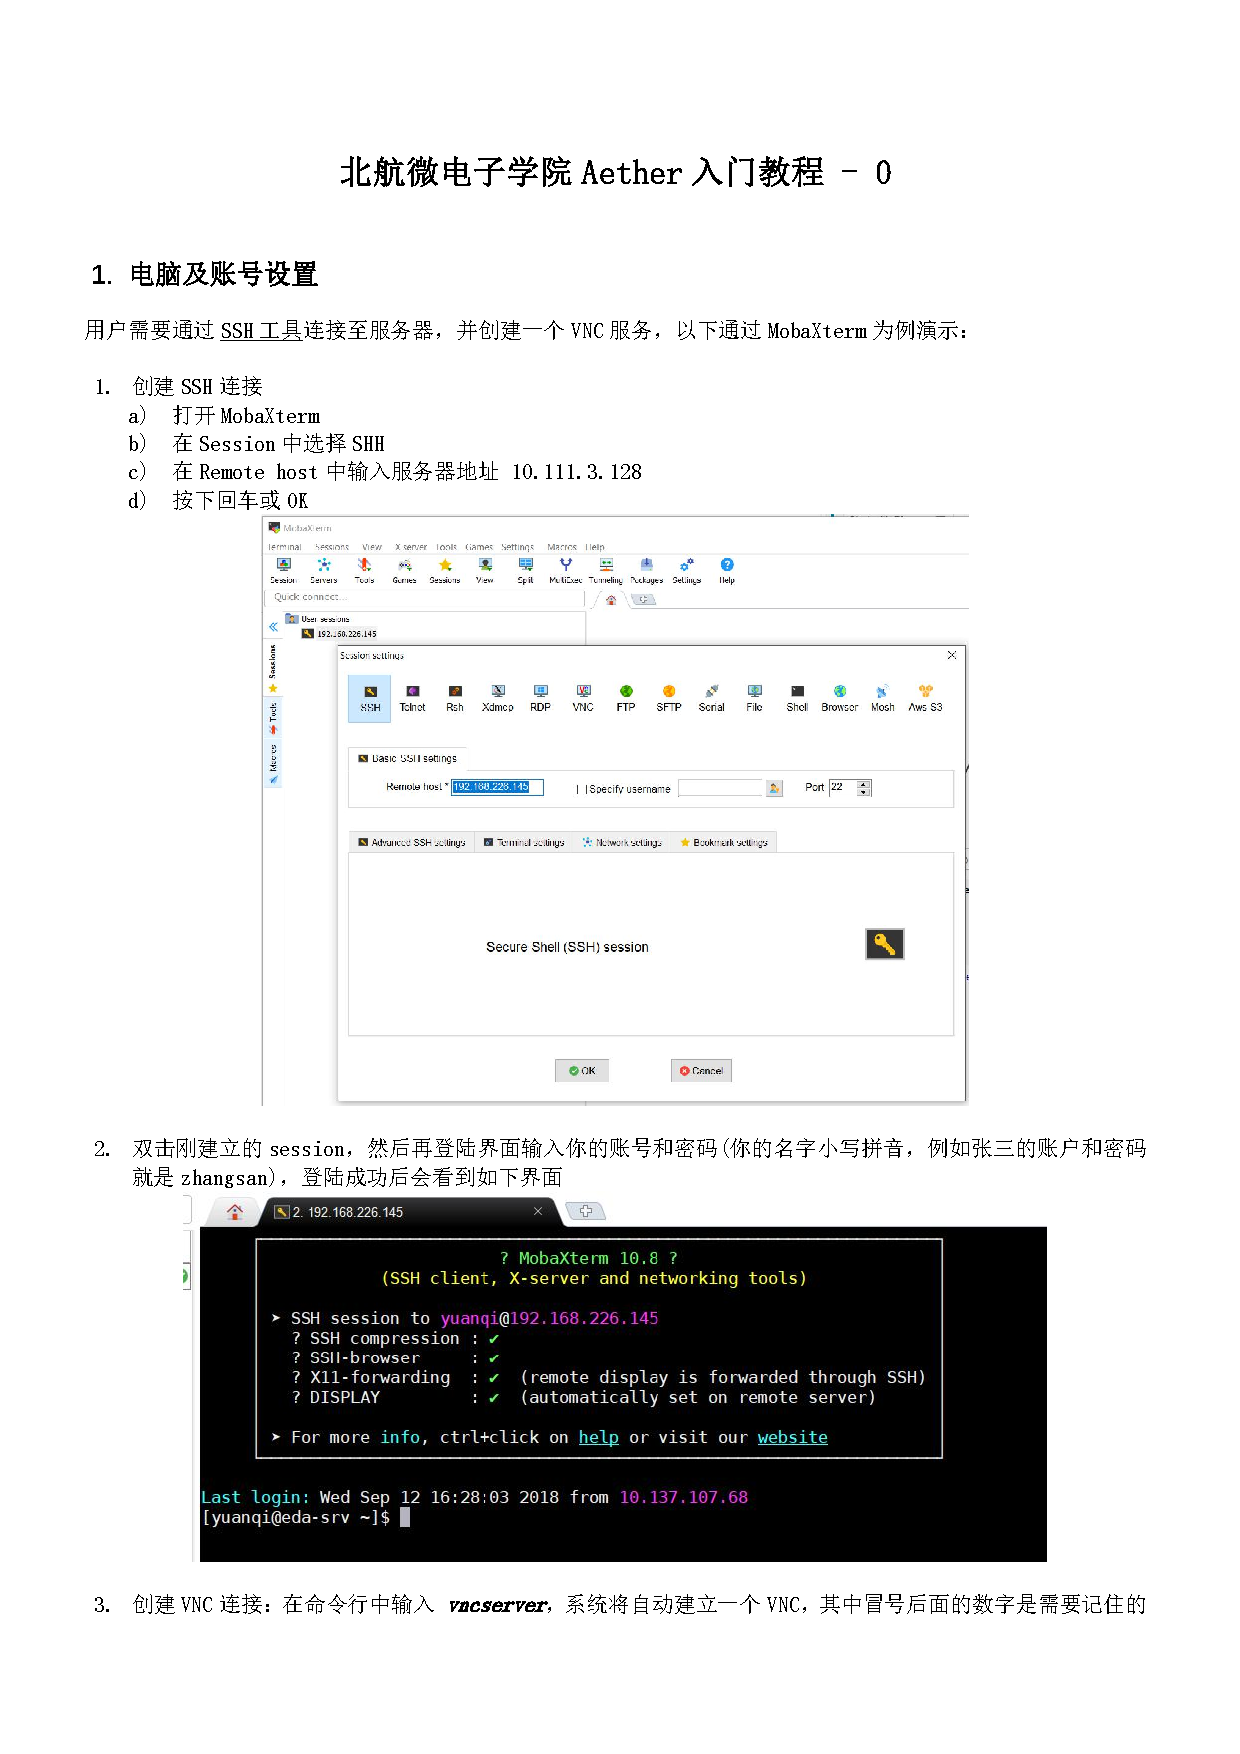
\includepdf[pages=-]{chap/tut1.pdf} 


\chapter{Aether DC 仿真}

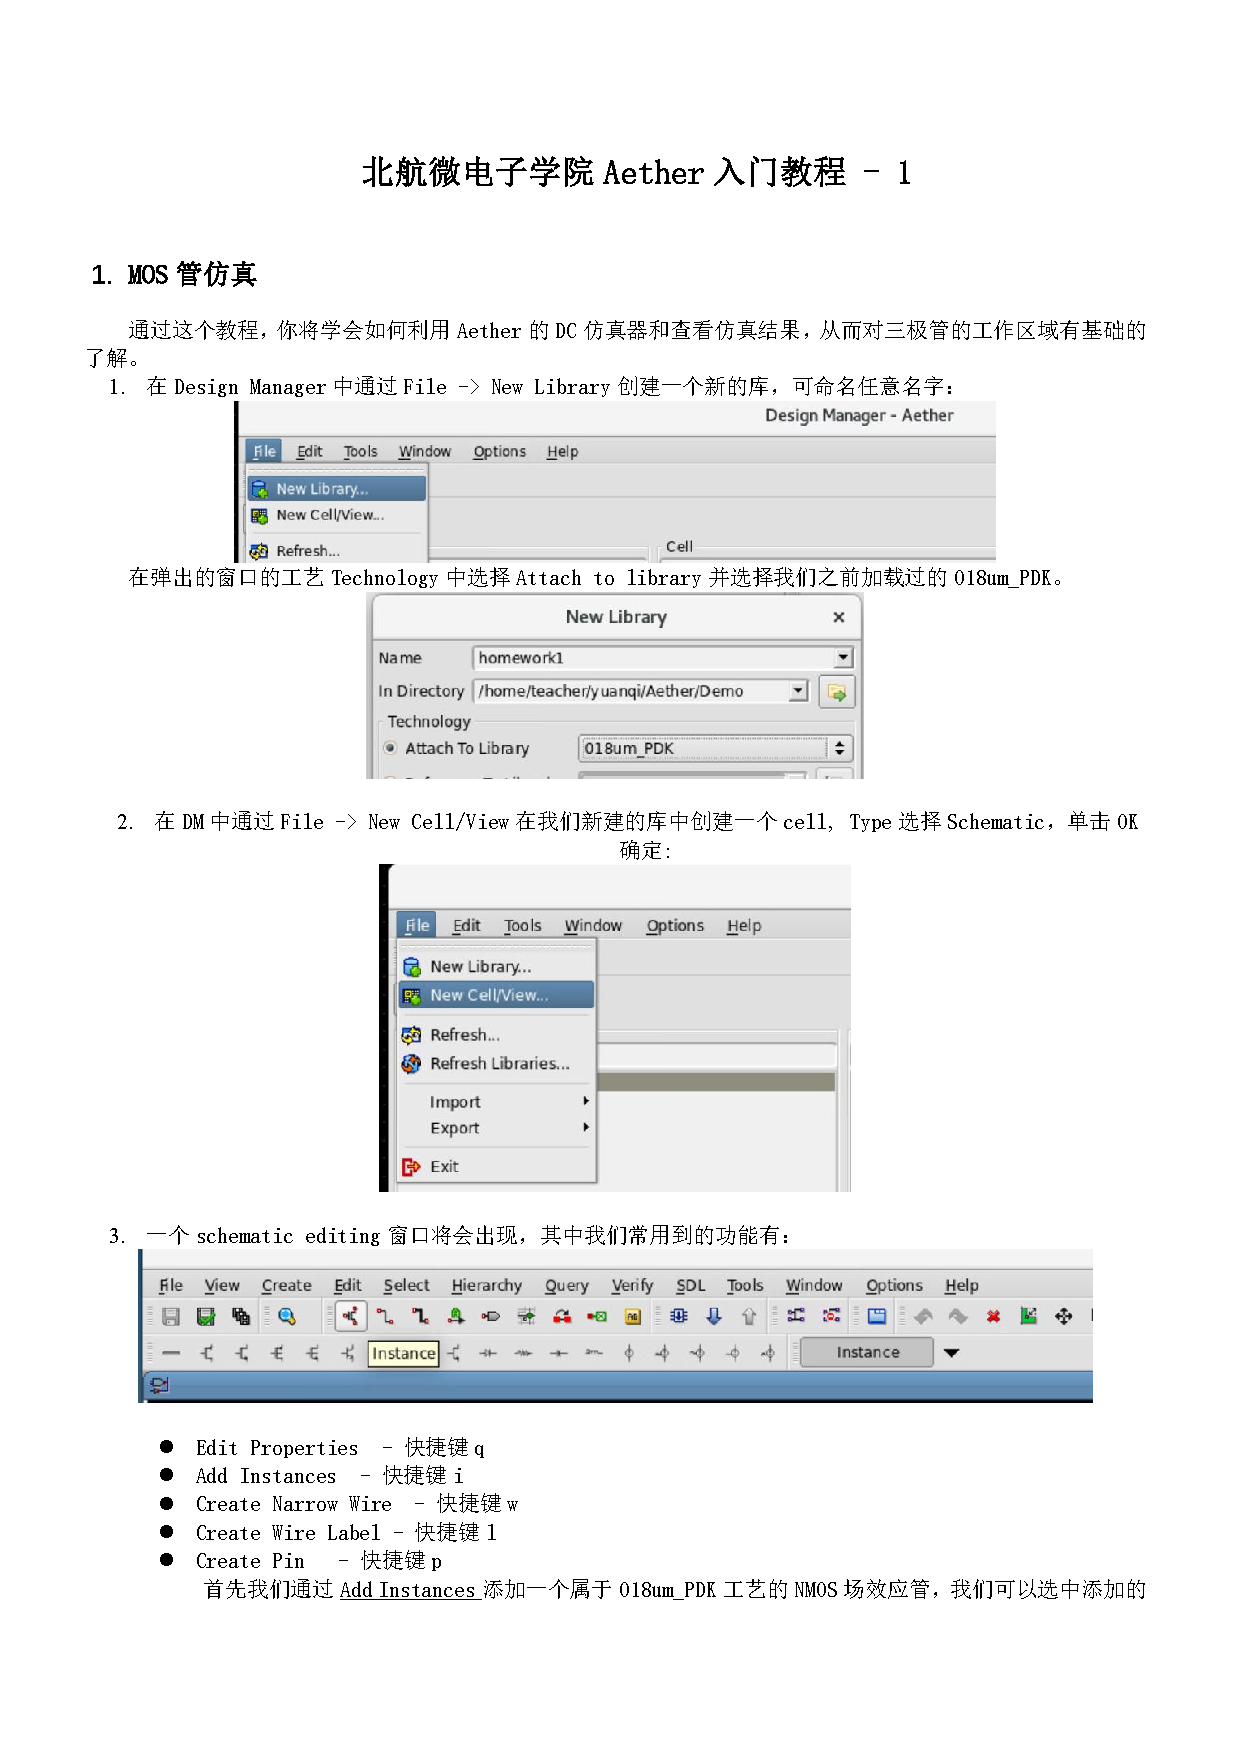
\includepdf[pages=-]{chap/tut2.pdf} 

\chapter{Aether AC/OP 仿真}

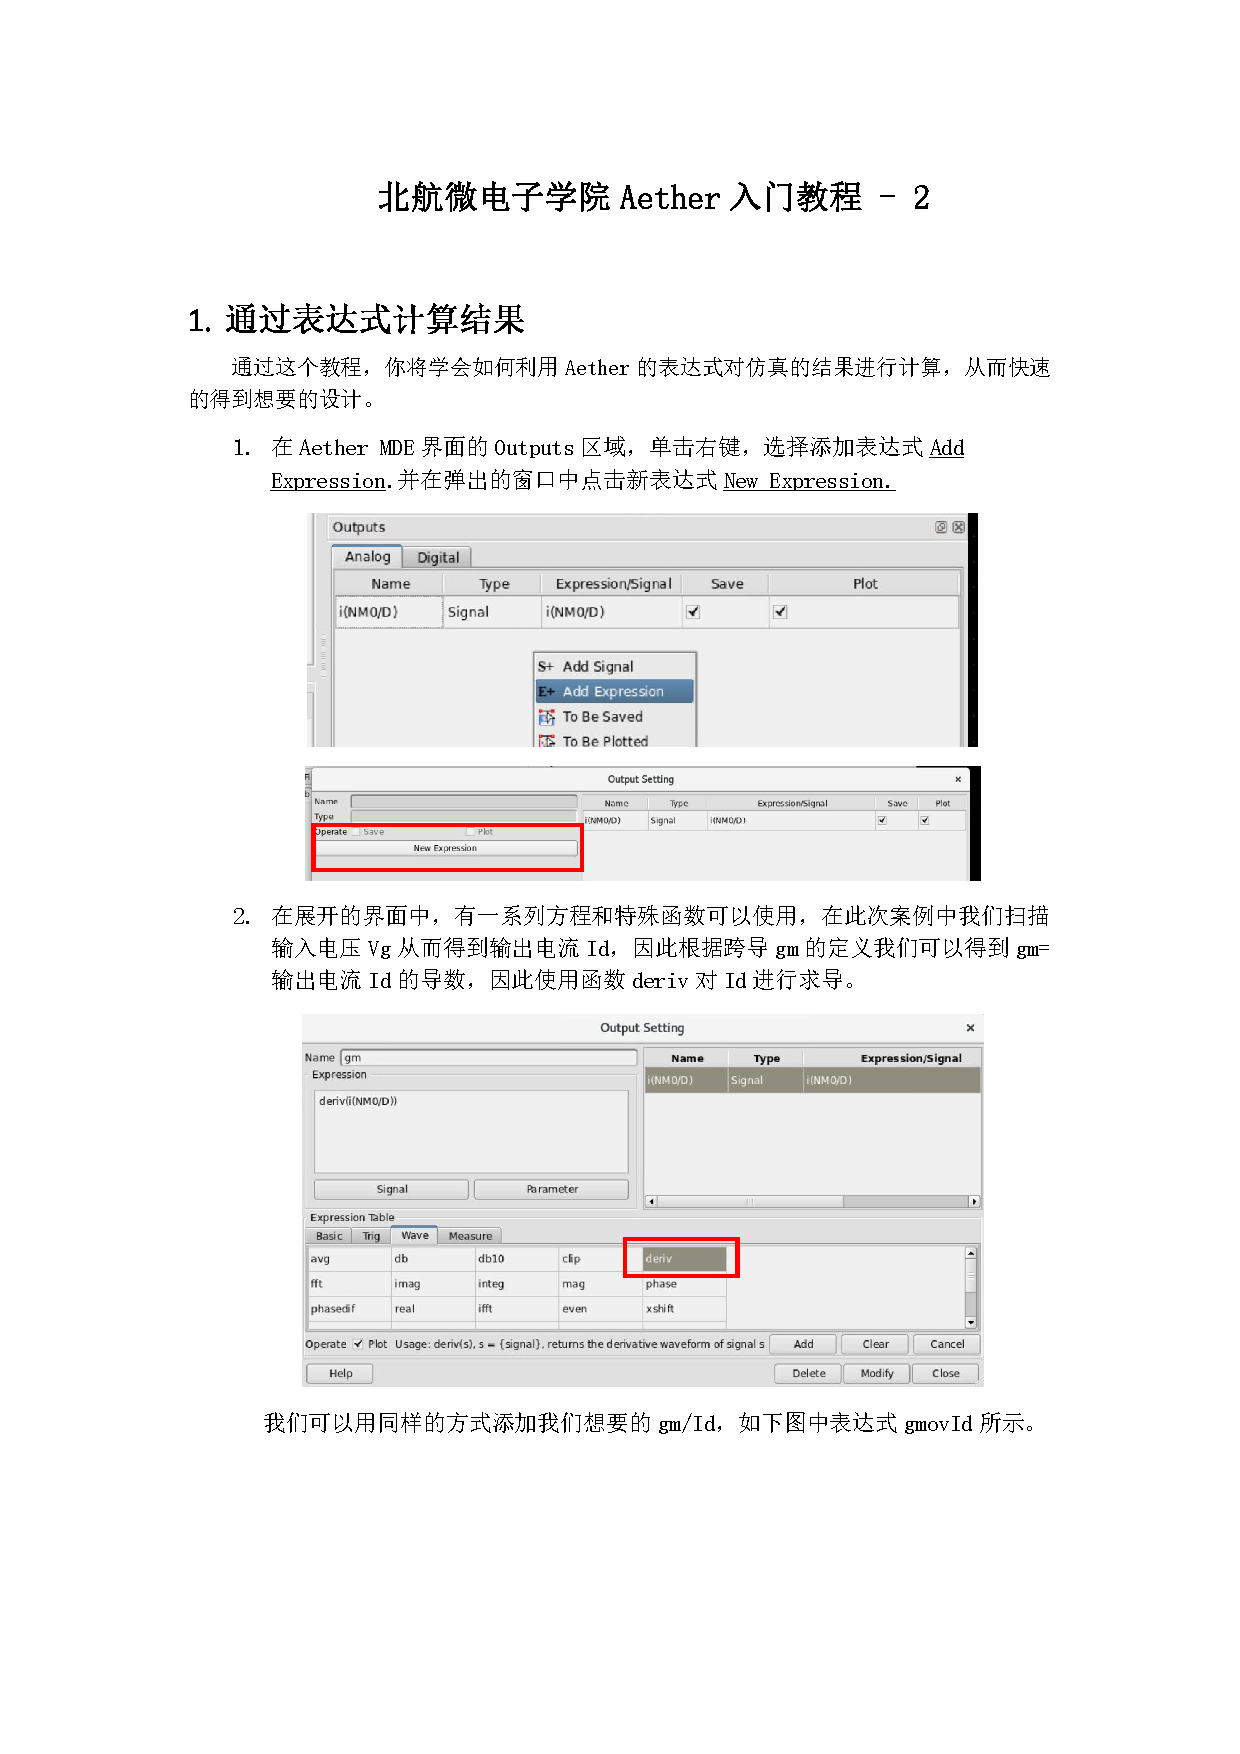
\includepdf[pages=-]{chap/tut3.pdf} 

\chapter{Aether NOISE 仿真}

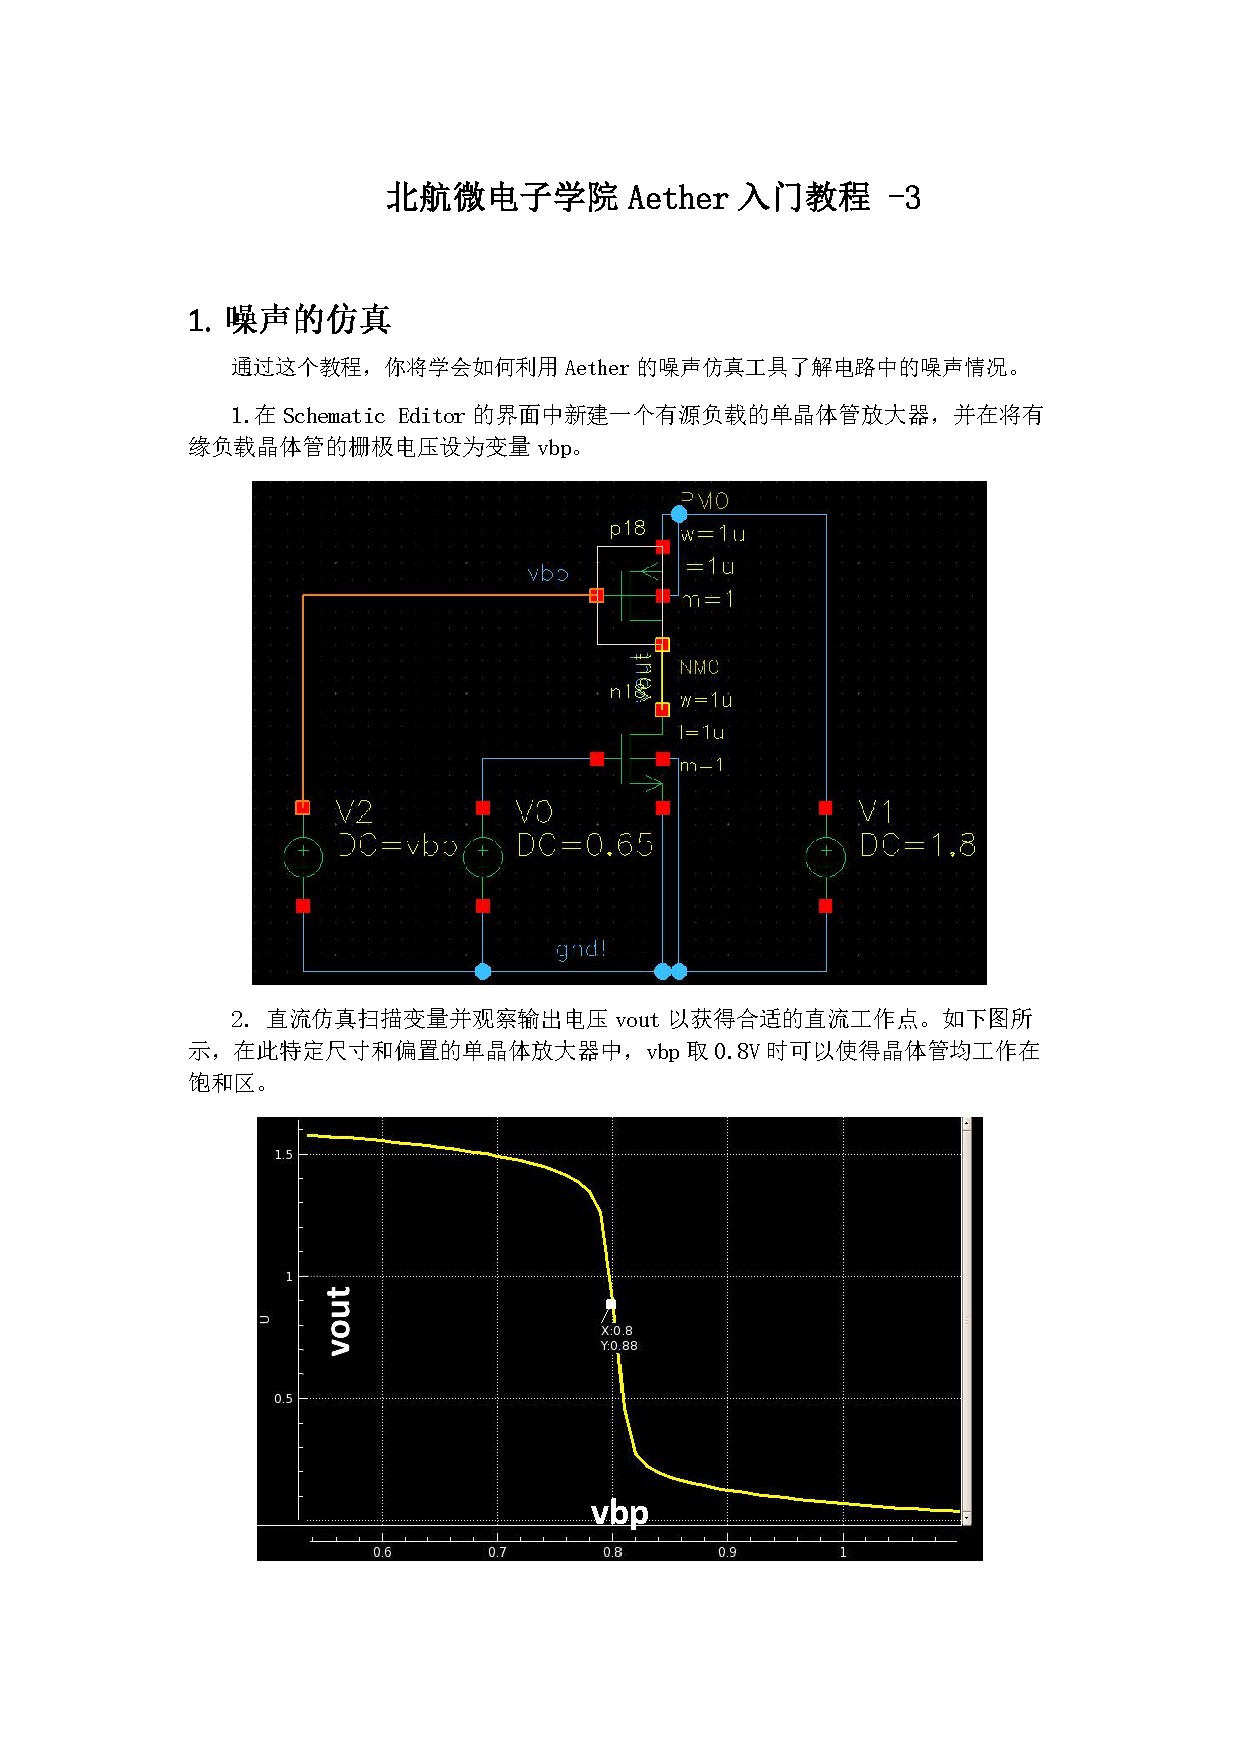
\includepdf[pages=-]{chap/tut4.pdf} 


\chapter{Aether 失调/蒙特卡洛/CMRR 仿真}

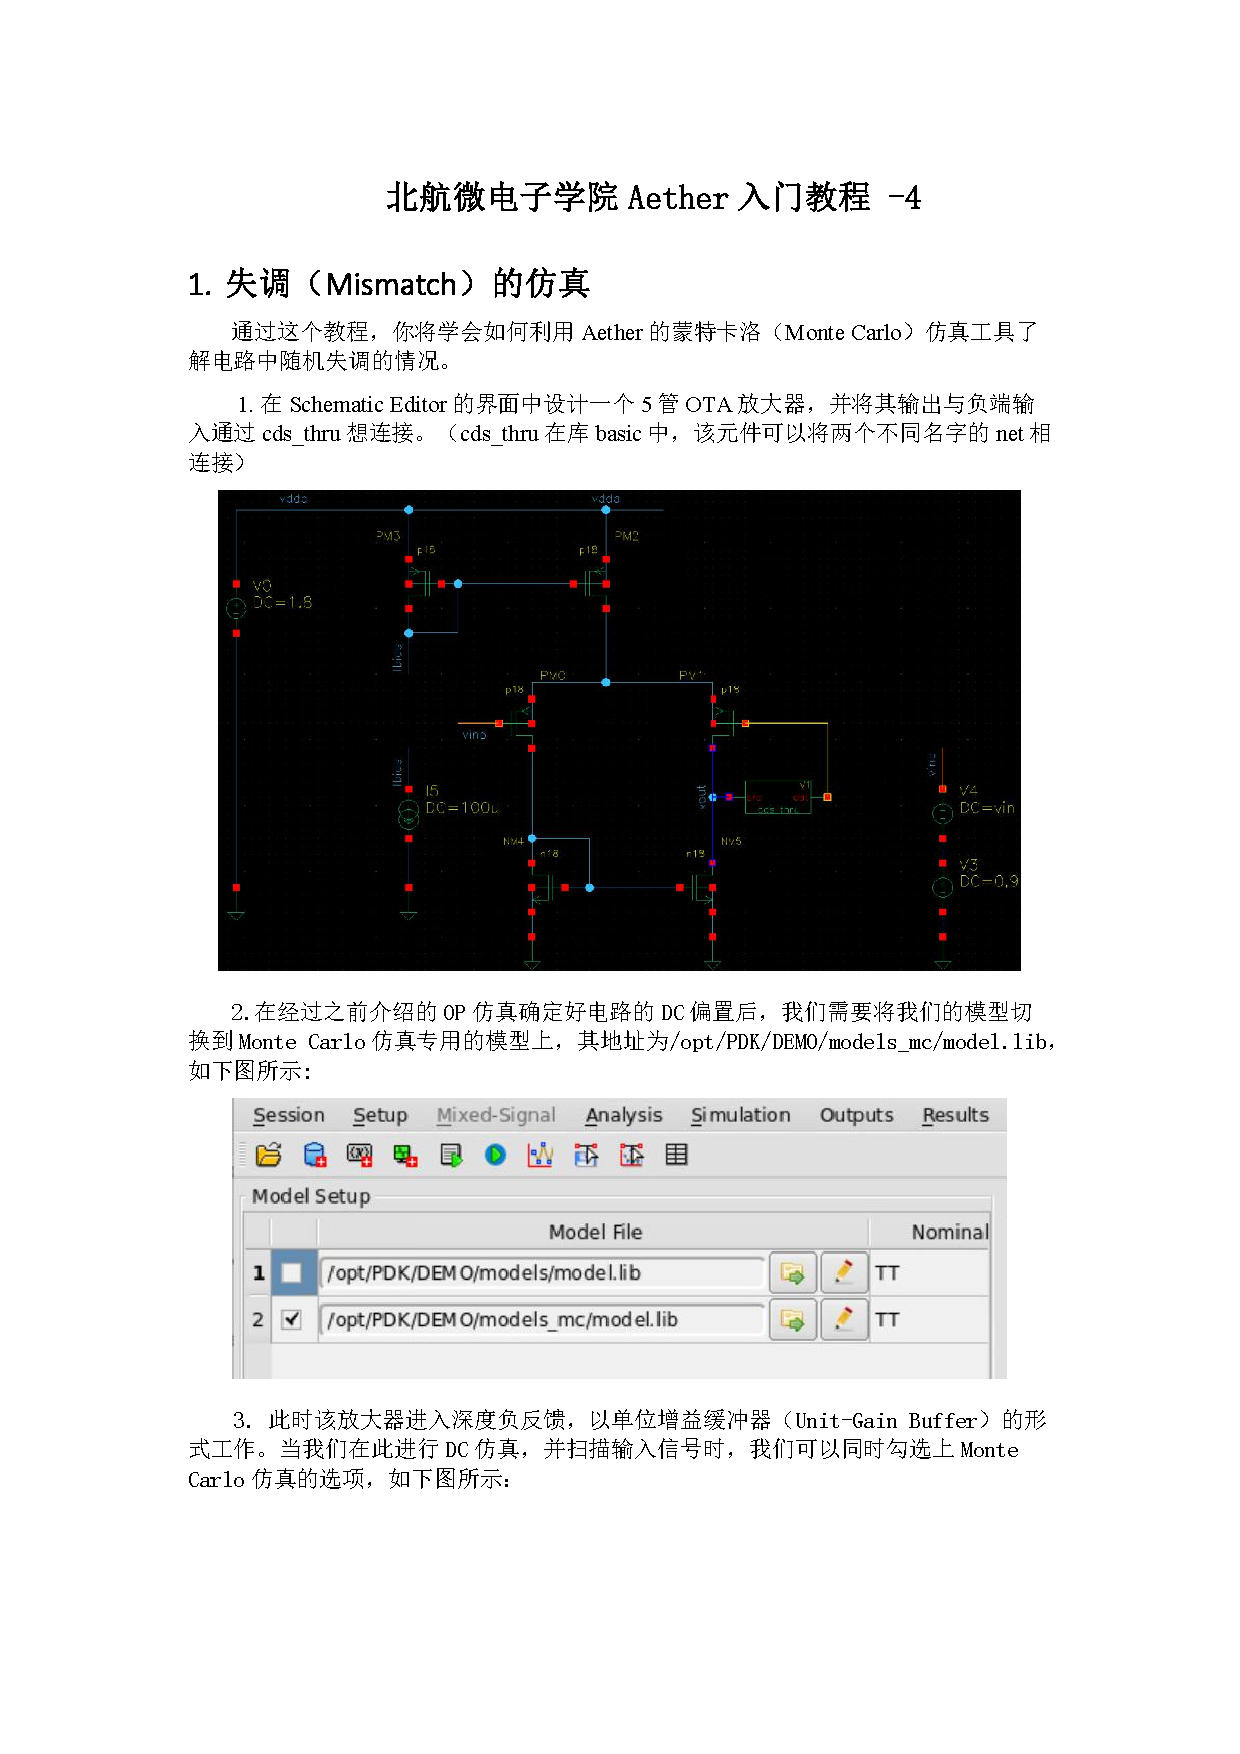
\includepdf[pages=-]{chap/tut5.pdf} 



\chapter{Aether TRANS/封装 仿真}

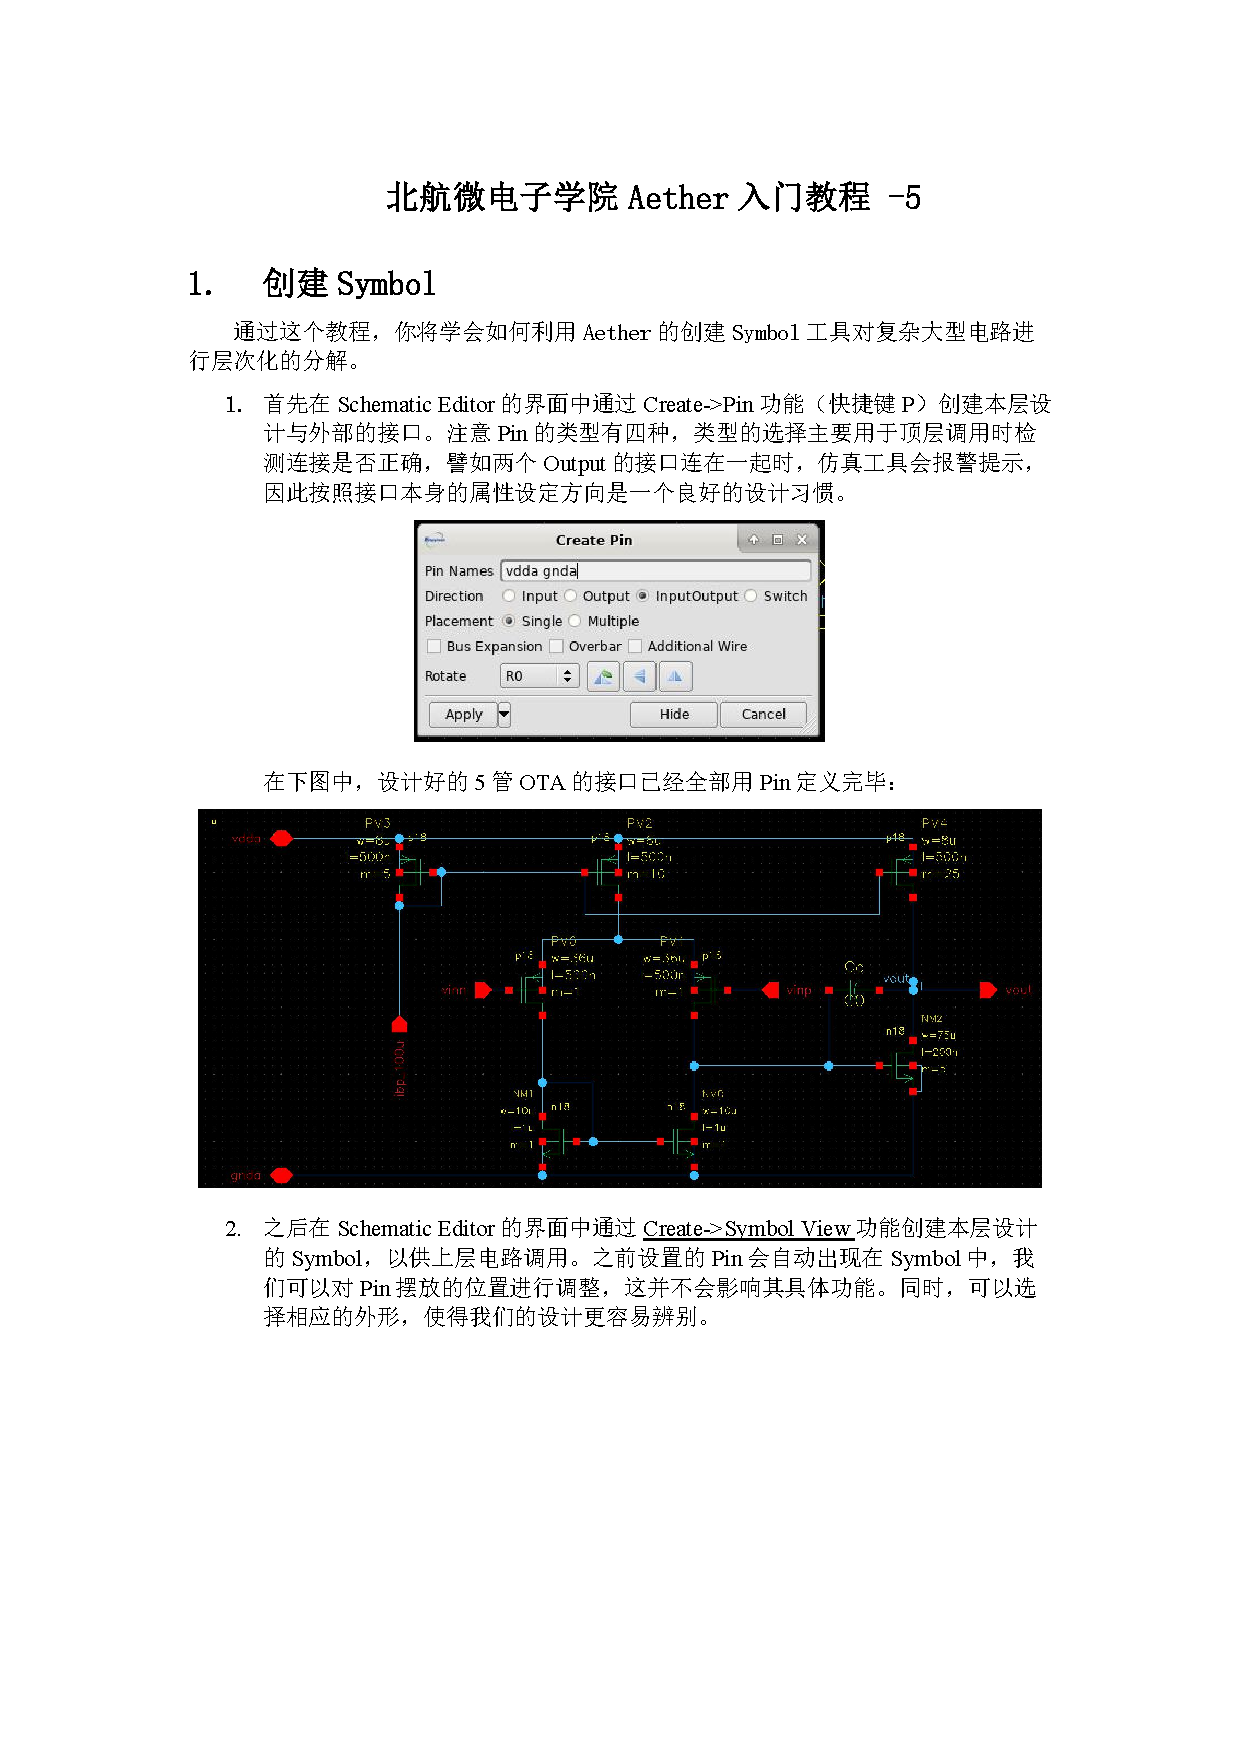
\includepdf[pages=-]{chap/tut6.pdf} 



\chapter{Aether 数摸混合 仿真}

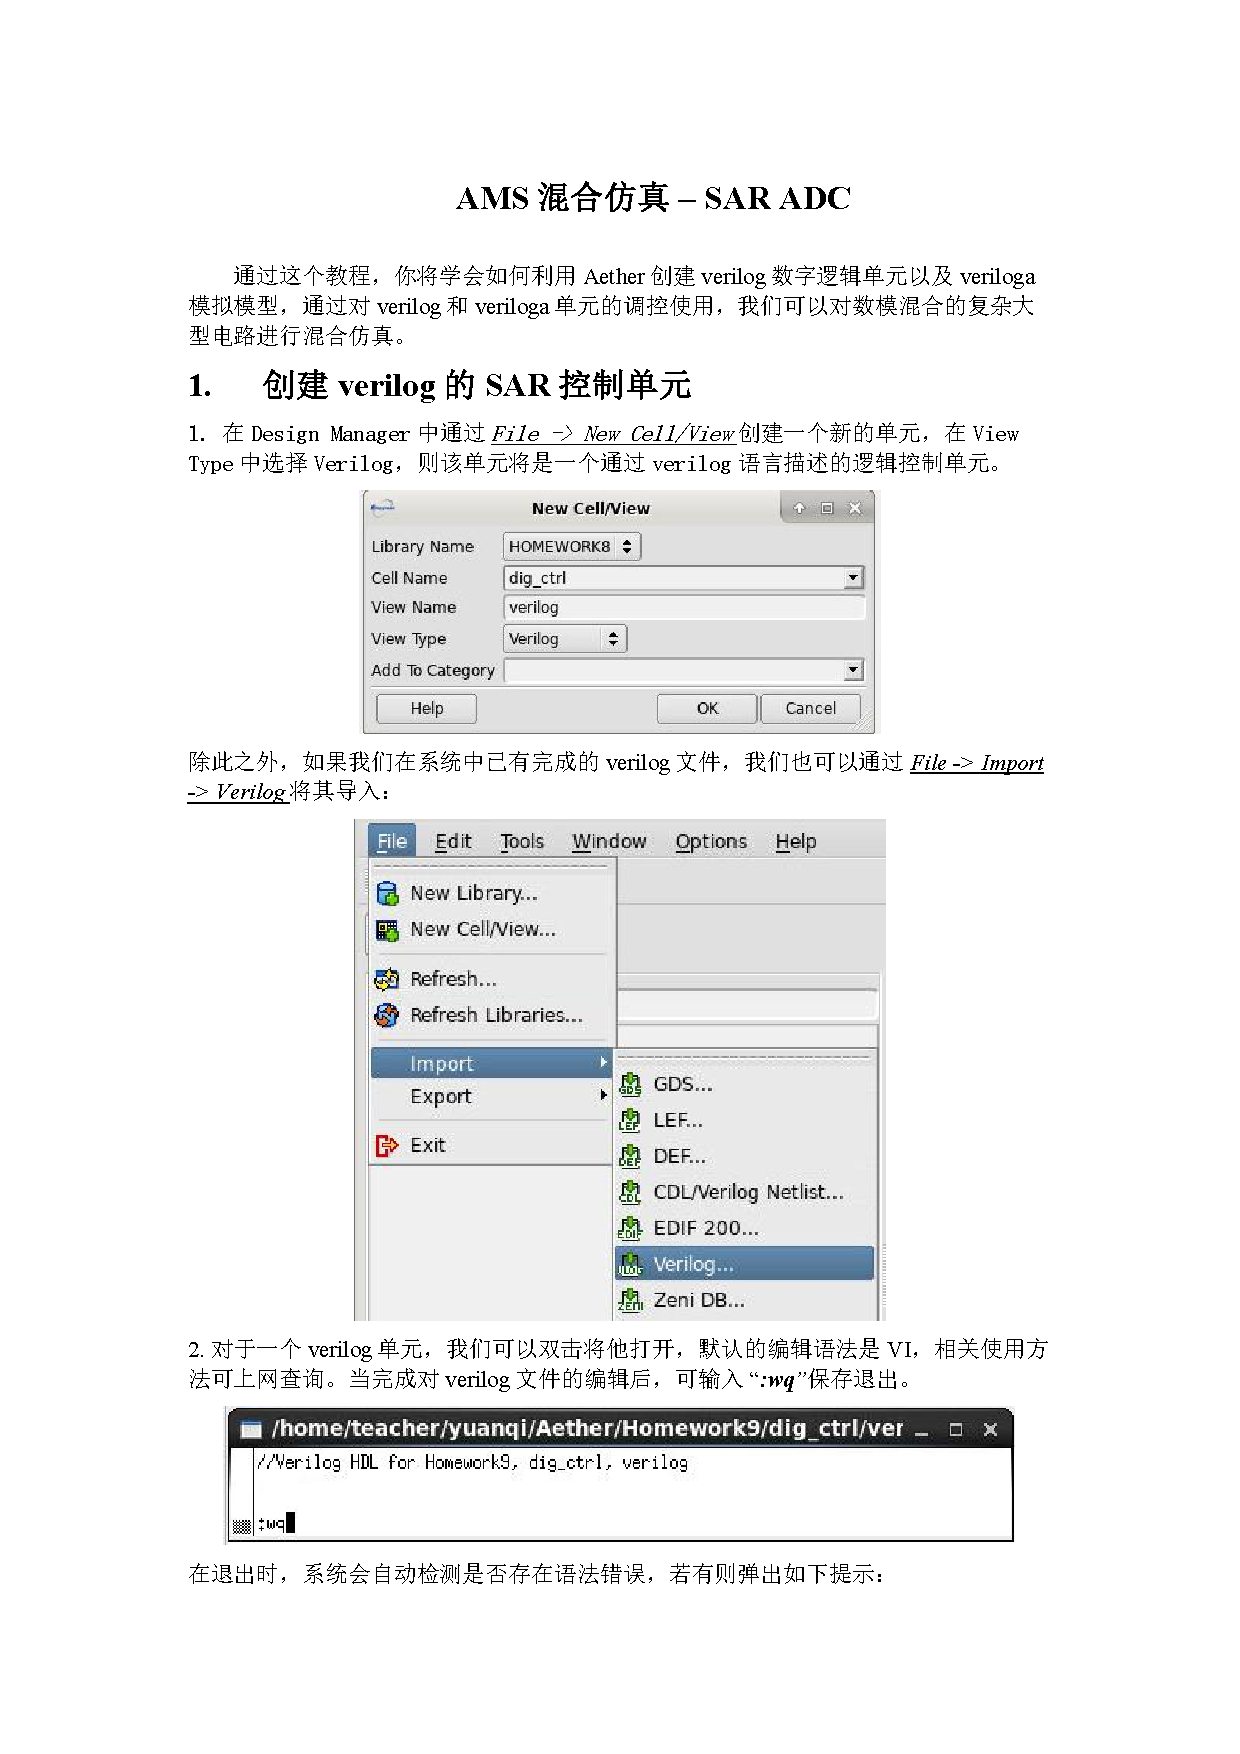
\includepdf[pages=-]{chap/tut7.pdf} 










\end{document}
